%%
%% licence       kaneton licence
%%
%% project       kaneton
%%
%% file          /home/mycure/kaneton/view/exams/arch-mips/2006/arch-mips-2006.tex
%%
%% created       julien quintard   [fri dec  2 22:25:51 2005]
%% updated       julien quintard   [sat dec  3 22:19:42 2005]
%%

%
% template
%

%%
%% licence       kaneton licence
%%
%% project       kaneton
%%
%% file          /home/buckman/kaneton/view/templates/exam.tex
%%
%% created       julien quintard   [fri dec  2 22:20:57 2005]
%% updated       matthieu bucchianeri   [sat feb 10 13:47:41 2007]
%%

%
% kaneton latex
%

%%
%% licence       kaneton licence
%%
%% project       kaneton
%%
%% file          /home/mycure/kaneton/view/papers/kaneton/kaneton.tex
%%
%% created       julien quintard   [thu dec  8 00:26:00 2005]
%% updated       julien quintard   [thu mar  2 13:59:43 2006]
%%

%
% template
%

%%
%% licence       kaneton licence
%%
%% project       kaneton
%%
%% file          /home/mycure/kaneton/view/templates/book.tex
%%
%% created       julien quintard   [wed mar  1 23:45:22 2006]
%% updated       julien quintard   [thu may  4 12:36:54 2006]
%%

%
% class
%

\documentclass[10pt,a4wide]{book}

%
% packages
%

\usepackage[english]{babel}
\usepackage[T1]{fontenc}
\usepackage{a4wide}
\usepackage{fancyheadings}
\usepackage{multicol}
\usepackage{indentfirst}
\usepackage{graphicx}
\usepackage{color}
\usepackage{xcolor}
\usepackage{verbatim}

\usepackage{aeguill}

\usepackage[Lenny]{../../../tools/latex/fncychap}

\pagestyle{fancy}

\setlength{\footrulewidth}{0.3pt}
\setlength{\parindent}{0.3cm}
\setlength{\parskip}{2ex plus 0.5ex minus 0.2ex}

%
% logos
%

\newcommand{\logos}
  {
    \begin{center}
      \includegraphics[scale=0.8]{../../logos/kaneton.pdf}
    \end{center}
  }

%
% colors
%

\definecolor{functioncolor}{rgb}{0.40,0.00,0.00}
\definecolor{commandcolor}{rgb}{0.00,0.00,0.40}
\definecolor{verbatimcolor}{rgb}{0.00,0.40,0.00}
\definecolor{noticecolor}{rgb}{0.87,0.84,0.02}

%
% function
%

\newcommand\function[3]{
  \begin{tabular}{p{0.2cm}p{13.8cm}}
  & {\color{functioncolor}\textbf{#1}}#2
  \end{tabular}

  \begin{tabular}{p{1cm}p{13cm}}
  & #3
  \end{tabular}}

%
% align
%

\newcommand\align[1]{
  \\ & \hspace{#1}}

%
% argument
%

\newcommand\argument[1]{\textit{#1}}

%
% command
%

\newcommand\command[2]{
  \begin{tabular}{p{0.2cm}p{13.8cm}}
  & {\color{commandcolor}\textbf{#1}}
  \end{tabular}

  \begin{tabular}{p{1cm}p{13cm}}
  & #2
  \end{tabular}}

%
% notice
%

\newcommand\notice[1]{
  {\color{noticecolor}\textbf{Notice}}

  \begin{tabular}{p{0.2cm}p{13.8cm}}
  & #1
  \end{tabular}}

%
% example
%

\newcommand\example[1]{
  \textit{Example:}

  \begin{tabular}{p{0.2cm}p{13.8cm}}
  & \textit{#1}
  \end{tabular}}

%
% warning XXX
%

%
% verbatim stuff
%

\makeatletter

\renewcommand{\verbatim@font}
  {\ttfamily\footnotesize\color{verbatimcolor}\selectfont}

\def\verbatim@processline{\hskip15ex\the\verbatim@line\par}

\makeatother

%
% header
%

\rhead{}
\rfoot{\scriptsize{The kaneton microkernel project}}

\date{\scriptsize{\today}}


%
% header
%

\lhead{\scriptsize{The kaneton microkernel project reference}}
\rhead{}

%
% title
%

\title{The kaneton microkernel reference
       \logos}

%
% authors
%

\author{\small{Julien Quintard},
        \small{Matthieu Bucchianeri},
        \small{Renaud Voltz}}

%
% document
%

\begin{document}

%
% title
%

\maketitle

%
% --------- text --------------------------------------------------------------
%

%
% authors
%

This document describes the kaneton microkernel reference project.

This document should be used by every student willing implement the
kaneton microkernel.

All the kaneton documents are available on the official website:
\textbf{http://www.kaneton.org}.

This document is under the \textbf{kaneton license}.

This document will reference the kaneton people by the word \textit{we}.

\newpage

The kaneton project was introduced at EPITA by two computer science
students:

\begin{itemize}
  \item
    Julien Quintard \footnote{quinta\_j@epita.fr}
  \item
    Jean-Pascal Billaud \footnote{billau\_j@epita.fr}
\end{itemize}

This document especially describes the kaneton reference microkernel
developed by:

\begin{itemize}
  \item
    Julien Quintard
  \item
    Matthieu Bucchianeri \footnote{bucchi\_m@epita.fr}
  \item
    Renaud Voltz \footnote{voltz\_r@epita.fr}
\end{itemize}

Nevertheless, many people contributed to this project and we thank them.

%
% toc
%

\tableofcontents

%
% chapters
%

XXX revoir ordre pour mieux introduire kaneton: design.pdf

%
% ---------- header -----------------------------------------------------------
%
% project       kaneton
%
% license       kaneton
%
% file          /home/mycure/kaneton/view/book/kaneton/goals.tex
%
% created       julien quintard   [fri jun  1 13:58:12 2007]
% updated       julien quintard   [mon may 19 23:09:48 2008]
%

%
% ---------- goals ------------------------------------------------------------
%

\chapter{Goals}
\label{chapter:goals}

In this chapter we will briefly introduce the kaneton microkernel
through the kaneton microkernel goals.

\newpage

%
% ---------- text -------------------------------------------------------------
%

The project was primarily designed by two students in computer science,
\name{Julien Quintard} and \name{Jean-Pascal Billaud}.

These two students previously actively contributed to the development
of a nanokernel-based operating system project in a French research laboratory.
This system was not powerful enough, especially from the design point of view.

Therefore, the two students started the design of a new microkernel
by their own, called \term{kaneton}, for educational purposes.

The design was based on five fundamental guidelines.

\begin{enumerate}
  \item
    \textbf{Educational}

    \-

    The kaneton project is built to become an educational project. The design
    as well as the implementation must therefore be as understandable as
    possible so that everyone interested in kernel internals can go through the
    documents and source code and actually understand how it works.

    \-

    This \textit{understandable} property can be achieved through a very clear
    and coherent design. Moreover, the implementation should be written using
    modern tools and techniques to make the code as generic as possible and
    easily readable.
  \item
    \textbf{Portability}

    \-

    The microkernel was particularly designed to be portable. The designers
    tried to develop a portability system powerful enough to port kaneton on
    any, existing or not, architectures.
  \item
    \textbf{Maintanability}

    \-

    Although microkernel-based operating systems rely on a modular design,
    kaneton designers also wanted the microkernel itself to be modular and
    maintainable.
  \item
    \textbf{Distributed Computing}

    \-

    The kaneton microkernel must be designed to fit distributed operating
    systems requirements. Indeed, the kaneton microkernel was developed in
    order to design and implement a distributed operating system named
    \term{kayou}.

    \-

    This point led to many specific choices in the kaneton microkernel design.
  \item
    \textbf{Demystification}

    \-

    kaneton people wanted to break some well-known kind of computer
    science rules. Indeed, for instance, many computer scientists consider
    the source code as the actual documentation. Also, for many low-level
    programmers, the kernel boot source code and more generally the
    kernel source code itself cannot be understandable, clear and coherent as
    it is related to low-level programming: microprocessor, devices \etc{}

    kaneton people paid particular attention to the microkernel source code to
    be easily understandable, maintainable and extendable. Moreover, kaneton
    people tried to write documentation for every part of the project.
\end{enumerate}

Notice that building an educational microkernel project is nothing innovative.
Indeed few other projects already exist; the most popular being \name{MINIX}
from \name{Vrije Universiteit}, \name{NachOS} from \name{Berkeley University}
or \name{PintOS} from \name{Stanford University}.

kaneton people tried to design and implement a modern microkernel since, the
original \name{MINIX} microkernel for example, do not use modern development
tools. Moreover, the kaneton source code is heavily commented and use modern
languages techniques while trying to stay easily understandable.

The educational characteristic of kaneton does not constraint it from being
optimised afterwards. kaneton people believe that implementing optimised
algorithms in the first place does not lead to maintainable implementations.

Finally, note that the kaneton project is actually composed of two projects:
the \name{kaneton microkernel \term{educational} project} which provides
everything necessary to students willing to learn about kernels internals;
and the \name{kaneton microkernel \term{research} project} which focuses on
designing and implementing a powerful, reliable, flexible microkernel.
Obviously these two projects are highly related as the kaneton educational
project relies on the implementation of the kaneton research project.

%%
%% licence       kaneton licence
%%
%% project       kaneton
%%
%% file          /home/mycure/kaneton/view/papers/kaneton/overview.tex
%%
%% created       matthieu bucchianeri   [mon jan 30 17:09:45 2006]
%% updated       julien quintard   [thu mar  2 13:12:22 2006]
%%

%
% overview
%

\chapter{Overview}

XXX ce chapitre va vous aider a reconnaitre les fonctionnalites principale
XXX d'un kernel dans kaneton.

The kaneton microkernel is only the core of an operating system.
Main tasks like hardware drivers or user services are implemented as
\textbf{servers}. So the microkernel only has a few functionalities to
provide:

\begin{itemize}
  \item
    Memory management.
  \item
    Process management.
  \item
    Communication.
  \item
    Events.
\end{itemize}

In this chapter we will describe briefly these tasks and all the
associated managers.

%
% memory management
%

\section{Memory Management}

Handling the memory -- from virtual address space to physical
addressing -- is done by three major managers, the \textbf{as},
\textbf{segment} and \textbf{region} managers.

%
% as
%

\subsection{as}

The address space manager just manages the different address spaces
used by the kaneton tasks.

In kaneton, we call an \textbf{as - address space} a list of memory
locations referenced by a task. Each task has its own address space.

%
% segment
%

\subsection{segment}

The segment manager just manages the segments reserved by
the different kaneton entities including the kernel, the drivers etc..

In kaneton terms a \textbf{segment} is a contiguous area of reserved
physical memory.

%
% region
%

\subsection{region}

The region manager keeps track of regions used to map segments for
each address space reserved on the system.

In kaneton, a \textbf{region} is contiguous area of virtual memory
mapping a segment's part.

%
% process management
%

\section{Process Management}

XXX

%
% communication
%

\section{Communication}

XXX

%
% events
%

\section{Events}

XXX

%%
%% copyright quintard julien
%% 
%% kaneton
%% 
%% development-environment.tex
%% 
%% path          /home/mycure/kaneton
%% 
%% made by mycure
%%         quintard julien   [quinta_j@epita.fr]
%% 
%% started on    Tue Jul  5 12:23:08 2005   mycure
%% last update   Sun Oct 23 02:55:45 2005   mycure
%%

%
% class
%

\documentclass[8pt]{beamer}

%
% packages
%

\usepackage{pgf,pgfarrows,pgfnodes,pgfautomata,pgfheaps,pgfshade}
\usepackage{colortbl}
\usepackage{times}
\usepackage{amsmath,amssymb}
\usepackage{graphics}
\usepackage{graphicx}
\usepackage{color}
\usepackage{xcolor}
\usepackage[english]{babel}
\usepackage{enumerate}
\usepackage[latin1]{inputenc}

%
% style
%

\usepackage{beamerthemesplit}
\setbeamercovered{dynamic}

%
% verbatim font
%

\definecolor{verbatimcolor}{rgb}{0,0.4,0}

\makeatletter
\renewcommand{\verbatim@font}
  {\ttfamily\footnotesize\color{verbatimcolor}\selectfont}
\makeatother

%
% new line
%

\newcommand{\nl}[0]{\vspace{0.4cm}}

%
% title
%

\title{Development Environment}

%
% authors
%

\author
{
  Julien~Quintard\inst{1} \\
  {\tiny julien.quintard@gmail.com}
}

\institute
{
  \inst{1} kaneton distributed operating system project
}

%
% date
%

\date{\today}

%
% logos
%

\pgfdeclareimage[interpolate=true,width=34pt,height=18pt]
                {epita}{../../logos/epita}
\pgfdeclareimage[interpolate=true,width=49pt,height=18pt]
                {upmc}{../../logos/upmc}
\pgfdeclareimage[interpolate=true,width=25pt,height=18pt]
                {lse}{../../logos/lse}

%
% table of contents at the beginning of each section
%

\AtBeginSection[]
{
  \begin{frame}<beamer>
   \frametitle{Outline}
    \tableofcontents[current]
  \end{frame}
}

%
% table of contents at the beginning of each subsection
%

\AtBeginSubsection[]
{
  \begin{frame}<beamer>
   \frametitle{Outline}
    \tableofcontents[current,currentsubsection]
  \end{frame}
}

%
% document
%

\begin{document}

%
% title frame
%

\begin{frame}
  \titlepage

  \begin{center}
    \pgfuseimage{epita} \hspace{0.1cm} \pgfuseimage{upmc} \hspace{0.1cm}
    \pgfuseimage{lse} \hspace{0.1cm}
  \end{center}
\end{frame}

%
% outline frame
%

\begin{frame}
  \frametitle{Outline}
  \tableofcontents
\end{frame}

%
% overview
%

\section{Overview}

% 1)

\begin{frame}
  \frametitle{Introduction}

  From the previous years, a development environment was introduced.

  \nl

  The questions are:

  \begin{enumerate}[<+->]
    \item
      Why?
    \item
      What are the advantages and disadvantages of such a
      development environment?
    \item
      How did the other promotions do?
  \end{enumerate}
\end{frame}

% 2)

\begin{frame}
  \frametitle{Explanations}

  Over the years, the kaneton project evolved, starting with a very
  simple introduction to low-level programming, to microkernel
  development and finally to a distributed operating system project.

  \nl

  Going always further implies many modifications in the project
  including:

  \begin{itemize}[<+->]
    \item
      The courses given which now go from the Intel processor to
      the distributed operating system concepts
    \item
      The assignments which always evolve to study advanced topics
    \item
      The context because we now have to provide parts of the microkernel
      to avoid students a development from scratch
    \item
      .. and so the requirements
  \end{itemize}
\end{frame}

% 3)

\begin{frame}
  \frametitle{The Courses}

  The kaneton project now comes with four courses:

  \begin{enumerate}
    \item
      The design of the kaneton distributed operating system including
      the microkernel
    \item
      The Intel processor
    \item
      The kernel concepts
    \item
      The distributed operating system concepts
  \end{enumerate}
\end{frame}

% 4)

\begin{frame}
  \frametitle{The Assignments}

  During the year 2005, the students develop a poor microkernel
  from scratch with few functionalities, a driver and finally a baby
  file system.

  \nl

  We cannot ask the students of the year 2006 to develop the same project
  but to go further to study advanced topics like distributed algorithms.

  \nl

  So, we cannot ask the students to develop every parts of the microkernel
  because this takes much time and implies to not study advanced
  topics.
\end{frame}

% 5)

\begin{frame}
  \frametitle{The Context}

  Providing students parts of the microkernel is not enough.

  \nl

  Indeed, we decided to provide a complete development environment
  including:

  \begin{itemize}
    \item
      Makefiles
    \item
      Shell scripts
    \item
      Papers
    \item
      Tools
    \item
      .. everything you need to start microkernel development
  \end{itemize}
\end{frame}

% 6)

\begin{frame}
  \frametitle{Why?}

  The remaining question is:

  \nl

  \textbf{Why providing such a development environment and not letting us
    develop one ourself?}

  \nl

  The answers simply are:

  \begin{itemize}
    \item
      Developing such a development environment takes much time and
      need experience
    \item
      This development environment include very powerful features:
      multiusers cooperation, different operating systems etc..
    \item
      Finally, students will not be able to create such a complicated
      development tree so it is provided to not waste time.
  \end{itemize}
\end{frame}

% 7)

\begin{frame}
  \frametitle{The Requirements}

  The students starting the kaneton project should think that they
  will learn many many things during the year.

  \nl

  This year, we are trying to lead students to a distributed operating
  system.

  \nl

  This implies more concepts, algorithms and techniques to learn.

  \nl

  To do this we introduced more courses but the students will have
  to work hard to be able to success.
\end{frame}

% 8)

\begin{frame}[containsverbatim]
  \frametitle{Tree}

  \begin{center}

  \begin{verbatim}
    /
      conf/
      core/
      doc/
      drivers/
      env/
      export/
      libs/
      papers/
      programs/
      services/
      tools/
  \end{verbatim}

  \end{center}
\end{frame}

%
% conf
%

\section{conf}

% 1)

\begin{frame}
  \frametitle{Overview}

  The \textbf{conf} directory contains user variables used to parameterise:

  \begin{itemize}
    \item
      the development environment: makefiles, scripts etc..
    \item
      the kernel
  \end{itemize}

  \nl

  This configuration system is very interesting coupled with versionning
  system.

  \nl

  Indeed, you can develop using special compilation flags, specific kernel
  configuration without conflicts with other developers.
\end{frame}

% 2)

\begin{frame}[containsverbatim]
  \frametitle{Tree}

  \begin{verbatim}
    conf/
      mycure/
        conf.c
        conf.h
        kaneton.conf
        modules.conf
        mycure.conf
      pwipwi/
      chiche/
  \end{verbatim}

  This configuration system uses the shell variable \$USER to find
  the main configuration file: \textbf{conf/\$USER/\$USER.conf}.
\end{frame}

% 3)

\begin{frame}
  \frametitle{conf.c}

  This file is not used yet.
\end{frame}

% 4)

\begin{frame}
  \frametitle{conf.h}

  This file contains macros to configure the kernel:

  \begin{itemize}
    \item
      \textbf{CONF\_TITLE}
    \item
      \textbf{CONF\_VERSION}
    \item
      \textbf{CONF\_DEBUG}
    \item
      etc..
  \end{itemize}

  \nl

  This file is included by the kernel code.
\end{frame}

% 5)

\begin{frame}
  \frametitle{kaneton.conf}

  This configuration file is used to pass arguments at the runtime to the
  servers.

  \nl

  This file is also used to configure kernel and servers input variables.
\end{frame}

% 6)

\begin{frame}
  \frametitle{modules.conf}

  This file contains the list of the modules to be loaded by the
  multi-bootloader.

  \nl

  These modules will be passed to the kernel at the boot time.

  \nl

  Be careful, a module here is not a module in the Linux or BSD terms.

  \nl

  A module is simply a file to load.
\end{frame}

% 7)

\begin{frame}
  \frametitle{\$USER.conf}

  Finally the main configuration file contains the configuration
  variables for the development environment.

  \nl

  This file uses the syntax of the make files.

  \nl

  Every variable defined in this file will be used by the makefiles
  and the scripts.
\end{frame}

%
% env
%

\section{env}

% 1)

\begin{frame}
  \frametitle{Overview}

  The \textbf{env} directory contains the different development environments.

  \nl

  This directory is the heart of the kaneton development system.

  \nl

  Indeed, a user can develop the kaneton project on a Mac machine using
  cross compilation for Intel processors ('cause PowerPC processor)
  while another one is using a FreeBSD operating system on an Intel processor.

  \nl

  So, the development environment has to deal with these different operating
  systems and architectures just for the development.
\end{frame}

% 2)

\begin{frame}
  \frametitle{Our System}

  To do this, we decided to introduce an environment system.

  \nl

  Every time a user gets the kaneton development tarball, he first has to
  create his development environment given a couple operating system and
  architecture which leads to an environment.

  \nl

  Once the environment is installed, the user can develop, compile the kernel
  etc.. without problems because everything (makefiles, scripts etc..) use
  the binaries, variables etc.. for his environment.

  \nl

  The environment is specified in the user configuration file.
\end{frame}

% 3)

\begin{frame}[containsverbatim]
  \frametitle{Tree}

  \begin{verbatim}
    env/
      clean.sh
      init.sh
      unix/
        clean.sh
        init.sh
        kaneton.mk
      macos-powerpc.ia32/
  \end{verbatim}

  \nl

  Here the \textbf{unix} is considered as the generic unix
  environment but everyone can add a specific linux, FreeBSD, Solaris etc..
  environment.
\end{frame}

% 4)

\begin{frame}
  \frametitle{init.sh}

  The \textbf{init.sh} shell script is used to install the development
  environment.

  \nl

  This script first gets the configuration variables from the user
  configuration file, then calls the specific \textbf{init.sh} script
  of the given environment.

  \nl

  Finally the script installs some links and initialises the makefile
  dependencies.

  \nl

  The \textit{[environment]}/init.sh shell script is used to install
  specific stuff.
\end{frame}

% 5)

\begin{frame}
  \frametitle{clean.sh}

  The \textbf{clean.sh} shell script just cleans the environment.

  \nl

  This shell script also call the environment specific clean.sh script.
\end{frame}

% 6)

\begin{frame}
  \frametitle{kaneton.mk}

  The \textbf{kaneton.mk} makefile dependency is the heart of the
  kaneton compilation system.

  \nl

  Indeed, every makefile is composed of calls to special routines
  which are implemented by the makefile dependency depending on the
  environment: operating system plus architecture source and destination.

  \nl

  Moreover the \textbf{kaneton.mk} makefile dependency includes the
  user configuration file so each makefile of the system is able to
  use user defined variables.

  \nl

  The kaneton compilation system uses a very special gmake feature:
  the makefile \textbf{call} function.
\end{frame}

% 7)

\begin{frame}[containsverbatim]
  \frametitle{Use}

  \begin{verbatim}
    $ make init
    [+] installing environment

    [+] your current configuration:
    [+]   environment:              unix
    [+]   architecture:             ia32
    [+]   multi-bootloader:         grub

    [...]

    $ make clean
    [+] cleaning environment

    [...]

    $ 
  \end{verbatim}
\end{frame}

%
% tools
%

\section{tools}

% 1)

\begin{frame}
  \frametitle{Overview}

  The \textbf{tools} directory contains programs, scripts, special
  files used by the kaneton project.

  \nl

  For example a script to initialise and install modules on a grub
  bootloader boot device is provided in the subdirectory
  \textit{scripts/multi-bootloaders/grub/}.

  \nl

  The \textbf{tools} directory also contains the ld scripts used
  to correctly compile the bootstrap, the bootloader, the kernel, the
  drivers, the services and the programs.
\end{frame}

% 2)

\begin{frame}[containsverbatim]
  \frametitle{Tree}

  \begin{verbatim}
    tools/
      scripts/
        ld/
          arch/
            ia32/
              bootstrap.lds
              bootloader.lds
              kaneton.lds
              driver.lds
              service.lds
              user.lds
        multi-bootloaders/
          grub/
          lilo/
        prototypes/
          mkp.py
  \end{verbatim}
\end{frame}

% 3)

\begin{frame}[containsverbatim]
  \frametitle{Use}

  \begin{verbatim}
    $ make build
    [+] initialising boot system

    [+] boot system initialised successfully
    $ make install
    [+] initialising boot system

    [+] /tmp/menu.lst
    [+] core/bootloader/bootloader
    [+] core/kaneton/kaneton
    [+] conf/mycure/kaneton.conf
    [+] drivers/cons/cons
    [+] services/dsh/dsh

    [+] boot system initialised successfully
    $ 
  \end{verbatim}
\end{frame}

% 4)

\begin{frame}[containsverbatim]
  \frametitle{Prototypes}

  The compilation system permits to generate the prototypes in a very easy
  and elegant way.

  \begin{verbatim}
    $ make proto
    [PROTOTYPES]            libdata.h
    [PROTOTYPES]            libstring.h
    [PROTOTYPES]            libsys.h
    [PROTOTYPES]            bootloader.h
    [PROTOTYPES]            ia32.h
    [PROTOTYPES]            kaneton.h
    [PROTOTYPES]            as.h
    [PROTOTYPES]            conf.h
    [PROTOTYPES]            serial.h

    [...]

    $ 
  \end{verbatim}
\end{frame}

% 5)

\begin{frame}[containsverbatim]
  \frametitle{Explanations}

  This system is based on tags in the header files which specify
  from which files to extract prototypes.

  \nl

  The tags are of the form:

  \begin{verbatim}
    /*
     * ---------- prototypes -------------------------------------------------
     *
     *      ../../kaneton/set/set.c
     *      ../../kaneton/set/set_array.c
     *      ../../kaneton/set/set_ll.c
     *      ../../kaneton/set/set_bpt.c
     */
  \end{verbatim}
\end{frame}

% 5)

\begin{frame}[containsverbatim]
  \frametitle{Dependencies}

  The compilation system uses full dependencies between files.

  \nl

  To regenerate the dependencies, for example when adding a
  \textit{\#include} c-preprocessor directive in a source file:

  \begin{verbatim}
    $ make dep
    [REMOVE]                .makefile.mk
    [DEPENDENCIES]          dump.c
    [DEPENDENCIES]          alloc.c
    [DEPENDENCIES]          sum2.c

    [...]

    $ 
  \end{verbatim}
\end{frame}

%
% libs
%

\section{libs}

% 1)

\begin{frame}
  \frametitle{Overview}

  The \textbf{libs} directory contains the libraries used by the kaneton
  project like:

  \begin{itemize}
    \item
      libc
    \item
      crt
    \item
      libposix
    \item
      etc..
  \end{itemize}
\end{frame}

%
% core
%

\section{core}

% 1)

\begin{frame}
  \frametitle{Overview}

  The \textbf{core} directory contains the source code for the microkernel
  including the bootstrap, the bootloader and the kernel itsef.

  \nl

  Each part contains an \textbf{arch} directory used for architecture
  dependent soure code.
\end{frame}

% 2)

\begin{frame}[containsverbatim]
  \frametitle{Tree}

  \begin{verbatim}
    core/
      bootstrap/
        arch/
          ia32/ <---;
          machdep --+
      bootloader/
        arch/
      kaneton/
        arch/
        as/
        conf/
        debug/
        id/
        segment/
        set/
        stats/
  \end{verbatim}
\end{frame}

%
% drivers
%

\section{drivers}

% 1)

\begin{frame}
  \frametitle{Overview}

  The \textbf{drivers} directory contains the drivers of the kaneton
  microkernel.

  \nl

  A driver, in the kaneton terms, is a microkernel server which is allowed
  to communicate with hardware devices.
\end{frame}

% 2)

\begin{frame}[containsverbatim]
  \frametitle{Tree}

  \begin{verbatim}
    drivers/
      cons/
        Makefile
        cons.c
      dma/
      kbd/
      ide/
  \end{verbatim}
\end{frame}

%
% services
%

\section{services}

% 1)

\begin{frame}
  \frametitle{Overview}

  The \textbf{services} directory contains the services of the kaneton
  microkernel.

  \nl

  A service, in the kaneton terms, in simply a server which does not
  communicate with the hardware.
\end{frame}

% 2)

\begin{frame}[containsverbatim]
  \frametitle{Tree}

  \begin{verbatim}
    services/
      dsh/
      mod/
        Makefile
        mod.c
        modfs.c
  \end{verbatim}
\end{frame}

%
% programs
%

\section{programs}

% 1)

\begin{frame}
  \frametitle{Overview}

  The \textbf{programs} directory contains the sources of common
  programs.

  \nl

  A program in the kaneton terms is just a non-privilegied
  process.
\end{frame}

% 2)

\begin{frame}[containsverbatim]
  \frametitle{Tree}

  \begin{verbatim}
    programs/
      ls/
      wc/
      cat/
      mount/
      umount/
      gcc/
      emacs/
  \end{verbatim}
\end{frame}

%
% export
%

\section{export}

% 1)

\begin{frame}
  \frametitle{Overview}

  The \textbf{export} directory is used to create kaneton distribution.

  \nl

  This feature is especially used by the maintainers of the kaneton
  project which create very special kaneton distribution for
  the students.
\end{frame}

% 2)

\begin{frame}[containsverbatim]
  \frametitle{Use}

  The only way to export kaneton is to do like this:

  \begin{verbatim}
    $ make export
    [!] usage: exporter.sh [stage]

    available stages: k0 k1 k2 k3 k4 k5 k6 k7 k8 k9 kaneton dist
    $ make export-k3
  \end{verbatim}

  \begin{itemize}
    \item
      \textbf{k[0-9]}: create a special kaneton version for the k[0-9]
      subproject
    \item
      \textbf{kaneton}: create an entire kaneton version for the lastest
      subproject
    \item
      \textbf{dist}: create an entire backup of the kaneton development
      project
  \end{itemize}
\end{frame}

%
% papers
%

\section{papers}

% 1)

\begin{frame}
  \frametitle{Overview}

  The \textbf{papers} directory contains the papers and lectures
  in relation with the kaneton project.

  \nl

  We prefered set the papers directly into the tarball so every student
  can easily read them.
\end{frame}

% 2)

\begin{frame}[containsverbatim]
  \frametitle{Tree}

  \begin{verbatim}
    papers/
      assignments/
      design/
      kaneton/
      seminar/
      lectures/
        kernels/
        inline-assembly/
        c-preprocessor/
        distributed-operating-systems/
        arch-ia32/
  \end{verbatim}
\end{frame}

% 3)

\begin{frame}[containsverbatim]
  \frametitle{Use}

  \begin{verbatim}
    $ make view
    [+] papers:

    [+]   assignments
    [+]   design
    [+]   arch-ia32
    [+]   c-preprocessor
    [+]   distributed-operating-systems
    [+]   inline-assembly
    [+]   kernels
    [+]   development-environment

    [!] usage: viewer.sh [paper]
    $ make view-design
  \end{verbatim}
\end{frame}

%
% doc
%

\section{doc}

% 1)

\begin{frame}
  \frametitle{Overview}

  The \textbf{doc} directory contains every document useful for
  the development of the kaneton project.

  \nl

  This directory will theorically contain documents on the different
  architectures, documents on some hardware devices like ide, usb etc..
\end{frame}

\end{document}

%
% ---------- header -----------------------------------------------------------
%
% project       kaneton
%
% license       kaneton
%
% file          /home/mycure/kaneton/view/book/development/source-tree.tex
%
% created       julien quintard   [thu may 17 22:41:36 2007]
% updated       julien quintard   [thu may 31 08:34:23 2007]
%

%
% ---------- source tree ------------------------------------------------------
%

\chapter{Source Tree}
\label{chapter:source tree}

In this chapter we will briefly describe the kaneton microkernel project
source tree.

\newpage

%
% ---------- text -------------------------------------------------------------
%

The kaneton microkernel reference source tree looks like the following
listing:

\begin{verbatim}
cheat/
configure/
environment/
export/
history/
kaneton/
library/
license/
test/
tool/
transcript/
view/
\end{verbatim}

%
% cheat/
%

\subsection*{cheat/}

Since the kaneton microkernel is implemented by students, the kaneton
people need to check whether students are cheating by re-using parts of
previous years projects or other kernel source codes available on the
\textit{Internet}.

To avoid cheating, kaneton people developed a software checking for
commonalities between different source codes.

This directory contains scripts that performs these verifications. However,
the students work over the years are not stored in this directory but in
the \textit{history/} directory instead.

%
% configure/
%

\subsection*{configure/}

This directory contains everything necessary for configuring its own
kaneton microkernel development environment through the compiling process
to the boot system.

Any new contributor should first look at this directory. However, note that
this directory mainly contains tools targeting final-users rather than
kaneton contributors. Indeed, for instance, the \textit{configure} utility
aims at providing a user-friendly way for configuration but does not take
advantage of the power of the kaneton development environment.

Contributors should then learn about how the development environment works
while final-users should use the \textit{configure} tool.

%
% environment/
%

\subsection*{environment/}

This directory contains everything necessary to the kaneton development
environment.

The kaneton development environment allows different developers to
interact on the development of the same microkernel in a pretty easy way.

The development environment aims at providing developers to possibility to
work in a collaborative manner without interfering with each other. These
developers are likely to run different operating systems on different
microprocessors. In addition, the kaneton microkernel can be targeted for
different microprocessor architectures. The development environment was
introduced to cope with these combinations by providing profiles, each
profile describing the behaviour of a component: underlying operating system,
target architecture, user-specific stuff etc.

As a result, each developer can use a different operating system and
microprocessor architecture with its own specific compiling flags, kaneton
parameters etc. without modifying another developer's configuration.

The development environment is detailed in \textit{Section
\ref{section:environment}}.

%
% export/
%

\subsection*{export/}

The \textit{export/} directory contains scripts used to generate a kaneton
tarball in order to be distributed to the students at the beginning of the
kaneton educational project.

Indeed, these scripts rearrange the kaneton hierarchy hidding some important
directories the students do not need to be aware of. Moreover some source
code parts are removed since the students have to rewrite these pieces
of code as assignments.

These scripts are also used for making backups and distribution tarbalss of
the kaneton microkernel.

%
% history/
%

\subsection*{history/}

The \textit{history/} directory contains the students work over the years
in the universities and schools the kaneton project was used as an operating
system course's implementation material.

The tools of the \textit{cheat/} directory use these students works for
performing cheating verifications.

%
% kaneton/
%

\subsection*{kaneton/}

This directory is the most important of the project since it contains
the whole microkernel source code.

The directory is composed of three important subdirectories: \textit{core/},
\textit{platform/} and \textit{architecture/}. These subdirectories are
described next.

% core/

\subsubsection*{core/}

This directory contains the kaneton core source code.

The directory is divided as shown below:

\begin{verbatim}
as/
region/
sched/
segment/
set/
task/
thread/
[...]
\end{verbatim}

Each directory represents a kaneton core manager. For more information on
the kaneton core, please refer to the appropriate document:
\textit{The kaneton microkernel :: core}

% platform/

\subsubsection*{platform/}

This directory contains everything in relation with what the kaneton
microkernel project calls a \textit{platform}. The platform represents the
board supporting the devices: microprocessor, memory, peripherals etc.

This directory obviously contains subdirectories for each platform
supported by the kaneton microkernel.

% architecture/

\subsubsection*{architecture/}

The \textit{architecture/} directory contains the source-code related to
the microprocessor architectures supported by the kaneton microkernel.

This directory is composed of subdirectories, each one representing a
supported architecture: \textit{ia32}, \textit{mips64} etc. Note that each
architecture can be specialised. For instance, the \textit{ia32/optimised}
architecture represents an optimised implementation of the \textit{Intel IA-32}
microprocessor architecture.

%
% library/
%

\subsection*{library/}

This directory contains the libraries used by the kaneton microkernel itself,
the kaneton microkernel servers or maybe both. This directory especially
contains the standard \textit{kaneton C library}.

%
% license/
%

\subsection*{license/}

This directory contains the licenses used for any program or document
in relation with the kaneton microkernel project. Indeed, the kaneton
microkernel is under the \textit{kaneton license} which is described in
depth in the documents contained in this directory. Note that these licenses
are also available in \textit{Chapter \ref{chapter:licenses}}.

Each student has to read and agree with the kaneton license before
implementing or even using the kaneton microkernel project..

Indeed, every user of the kaneton-related stuff is considered as having
implicitly accepted the kaneton license.

%
% test/
%

\subsection*{test/}

Since the kaneton microkernel is used as a material for operating system
courses, the kaneton microkernel reference, which is the basis of students
work, must be extremely reliable.

The kaneton project therefore contains a set of tools in order to validate
the kaneton reference implementation behaviour. These tools are also used
for evaluating the correctness of the students implementation.

The \textit{test/} directory contains the set of kaneton scripts and tests
for validating a kaneton microkernel implementation.

%
% tool/
%

\subsection*{tool/}

This directory contains additional scripts and configuration files used by
the kaneton development environment or the kaneton developers.

As examples, this directory contains scripts for generating prototypes,
building a boot device etc.

%
% transcript/
%

\subsection*{transcript/}

This directory contains real-time recorded sessions. These sessions can be
replayed in order to present a feature of the development environment or
of the kaneton microkernel.

%
% view/
%

\subsection*{view/}

This directory contains all the kaneton documents including kaneton
administrative documents, examinations, lectures materials, kaneton papers
and books etc.

Additionally, scripts are provided in order to very easily build and
display these documents.
%%
%% licence       kaneton licence
%%
%% project       kaneton
%%
%% file          /home/mycure/kaneton/view/papers/kaneton/coding-style.tex
%%
%% created       matthieu bucchianeri   [mon jan 30 17:32:57 2006]
%% updated       julien quintard   [thu mar  2 13:57:17 2006]
%%

%
% coding style
%

\chapter{Coding style}

The kaneton project developers try to follow a coding style. This
coding style was introduced to normalize the source code, leading to a
more readable source code.

Nevertheless, you can adapt this coding style to your own but try to
follow the rules.

%
% case
%

\section{Case}

The whole kaneton source code is written using lower case letters.

Moreover, every text including comments etc.. must be written using
lower case letters

%
% headers
%

\section{Headers}

Each file must start with an header formatted as shown below:

\begin{verbatim}
/*
 * licence       kaneton licence
 *
 * project       kaneton
 *
 * file          /home/mycure/kaneton/core/kaneton/as/as.c
 *
 * created       julien quintard   [fri feb 11 02:23:41 2005]
 * updated       matthieu bucchianeri   [mon jan 30 20:30:57 2006]
 */
\end{verbatim}

An emacs configuration file for automatically generating and updating
this header can be found in \textit{tools/emacs}.

Additionally, you need to set two environment variables to generate
a correct kaneton header:

\begin{itemize}
  \item
    \textbf{EC\_LICENCE} must be set to ``kaneton licence''.
  \item
    \textbf{EC\_DEVELOPER} must be set to your first name and last name.
\end{itemize}

Please, do not use nicknames in headers.

%
% naming convention
%

\section{Naming Convenions}

To keep the code as clear as possible, there are several conventions on
types, functions and variables naming.

%
% variables
%

\subsection{Variables}

Here are a few rules you are encouraged to follow:

\begin{itemize}
  \item
    \textbf{sz} suffix for variables representing a size.

    \begin{verbatim}
      #define PAGESZ          4096

      int                     modsz;
    \end{verbatim}
  \item
    \textbf{n} prefix for variables representing a number of objects.

    \begin{verbatim}
      int                     nclusters;
    \end{verbatim}
  \item
    etc..
\end{itemize}

Moreover, the types are used as pre-names:

\begin{verbatim}
t_vaddr                 video_vaddr;
\end{verbatim}

This example is not correct, instead prefer:

\begin{verbatim}
t_vaddr                 video;
\end{verbatim}

%
% functions
%

\subsection{Functions}

Function names must be prefixed by the file name, context name they are
implemented in.

For example, a function part of the address space manager must be prefixed
by \textit{as\_}.

These names must be chosen carefully: they must explicitely define
what the function does without being too long.

%
% types
%

\subsection{Types}

As variables and functions, type names must be expressed in english
with lower case letters.

Here are the prefixes you must use when writing your own types:

\begin{itemize}
  \item
    \textbf{m\_} for managers main structures.
  \item
    \textbf{o\_} for kaneton objects.
  \item
    \textbf{i\_} for interfaces.
  \item
    \textbf{d\_} for architecture-dependent structures.
  \item
    \textbf{s\_} for general purpose structures.
  \item
    \textbf{t\_} for basic and general purpose typedefs.
  \item
    \textbf{c\_} for kaneton capabilities.
  \item
    \textbf{u\_} for kaneton unique identifiers.
\end{itemize}

Notice that \textbf{d\_} can be combined with other prefixes, for
example \textbf{do\_} for a dependent object.

%
% includes
%

\section{Includes}

To keep the code clear and compact, developers only need to include a
minimal number of header files:

\begin{itemize}
  \item
    \textbf{kaneton.h} for the microkernel declarations.
  \item
    \textbf{klibc.h} for the kaneton specific C library.
\end{itemize}

These files are located in the include path, so do not use relative include
path.

\begin{verbatim}
#include <libc.h>
#include <kaneton.h>

int             main(int                argc,
                     char**             argv)
{
  [...]

  return (0);
}
\end{verbatim}

All include files must be protected against multiple inclusions. The
guard macro to use must be named using the directory name, one underscore,
the file name, one underscore and a capital ``H''.

For example, the file \textit{core/include/kaneton/segment.h} will be
guarded as follow:

\begin{verbatim}
#ifndef KANETON_SEGMENT_H
#define KANETON_SEGMENT_H	1

[...]

#endif
\end{verbatim}

In addition, for architecture-dependent files, the guard macro must begin
with the architecture name; for example for the Intel architecture:
\textit{IA32\_KANETON\_SEGMENT\_H}.

%
% types
%

\section{Types}

You may use as soon as possible standard types: \textbf{t\_uint8},
\textbf{t\_sint32}, \textbf{t\_uint64} etc..

This nomenclature is more understandable than
\textbf{unsigned long long int}.

%
% return values
%

\section{Return Values}

Every function must report whether it successed or failed.

In kaneton, functions' return type must be \textbf{t\_error}.

A function will return \textbf{ERROR\_NONE} on success and anything
else on error, for example \textbf{ERROR\_UNKNOWN} to indicate a non-specific
error.

%
% indentation
%

\section{Indentation}

There are several indentation rules in kaneton.

\begin{enumerate}
  \item
    Field names of structures and unions must be aligned with the
    structure or union name.

    \begin{verbatim}
      struct       s_set
      {
        u_set      id;
        t_setsz    size;
        t_type     type;
      };
    \end{verbatim}

    or

    \begin{verbatim}
      typedef struct
      {
        o_id       id;
        u_stats    stats;
        u_set      container;
      }            m_as;
    \end{verbatim}
  \item
    Macros and variables must be aligned as shown below:

    \begin{verbatim}
      #define TASK_PRIOR_CORE     230
      #define TASK_HPRIOR_CORE    250
      #define TASK_LPRIOR_CORE    210

      m_task*                     task;
      u_task                      ktask = ID_UNUSED;
    \end{verbatim}

    This rule also applies for variables declarations in functions.
  \item
    Function prototypes and bodies should look like this:

    \begin{verbatim}
      t_error             stats_function(u_stats          id,
                                         char*            function,
                                         t_stats_func**   f)
      {
        t_sint64          slot = -1;
        t_sint64          i;

        [...]
      }
    \end{verbatim}

    Notice that argument names are aligned between each other,
    and variable names are aligned with function name and between
    each other.

    Try to respect this alignment between functions in a single file:
    function names may be all aligned and argument names also.
\end{enumerate}

%
% comments
%

\section{Comments}

As kaneton is intended to be a pedagogical project with clear and
understandable source code; no need to say that comments take a very
important part of this objective.

Every file must begin with a comment describing what is done in this
code via the \textit{information} section.

Moreover, every function must be preceded by a comment defining its
behavior.

For complex functions and yo prevent direct comments in the source code,
we used \textbf{steps}:

\begin{itemize}
  \item
    Each critical code section in a function is preceded by a step
    number.
  \item
    The function header comment contains steps descriptions.
\end{itemize}

An example is present below:

\begin{verbatim}
/*
 * this function shows the usage of comments and steps.
 *
 * steps:
 *
 * 1) compute the index.
 * 2) make the operation.
 * 3) check the result.
 */

t_error         test_foobar(int      a,
                            int      b,
                            int*     c)
{
  int           index;

  /*
   * 1)
   */

  index = text_make_index(a, b);

  /*
   * 2)
   */

  index = index * a + b;

  /*
   * 3)
   */

  if (index < 0)
    return (ERROR_UNKNOWN);

  *c = index;

  return (ERROR_NONE);
}
\end{verbatim}

%
% sections
%

\section{Sections}

kaneton files are divided in multiple sections.

Section are delimited as shown below:

\begin{verbatim}
/*
 * ---------- includes ------------------------------------------------
 */
\end{verbatim}

Possible sections in a file are:

\begin{itemize}
  \item
    \textbf{header files}: information, dependencies, defines, types,
    prototypes, macros, etc..
  \item
    \textbf{source files}: information, extern, globals, includes,
    functions, etc..
  \item
    \textbf{make files}: dependencies, directives, variables, rules, etc..
\end{itemize}

Moreover, every important file, for example the main file of each
kaneton manager, have to contain a section \textit{information} describing
the whole manager.

In addition, a section named \textit{assignments} is generally necessary
for manager will be filled in by the students. This section briefly describes
the work to be done by the students.

%
% macros
%

\section{Macros}

The kaneton microkernel uses few fundamental macros lited below:

\begin{itemize}
  \item
    \textbf{\_\_\_bootloader} indicates that this source code belongs to
    the bootloader.
  \item
    \textbf{\_\_\_kernel} indicates that this source code belongs to the
    microkernel.
  \item
    \textbf{\_\_\_kaneton} indicates that this kernel is the kaneton
    microkernel.
  \item
    \textbf{\_\_\_wordsz} indicates the word size: 16-bit, 32-bit,
    64-bit etc..
  \item
    \textbf{\_\_\_endian} indicates the endianness.
\end{itemize}

%%
%% licence       kaneton licence
%%
%% project       kaneton
%%
%% file          /home/mycure/kaneton/view/papers/kaneton/core.tex
%%
%% created       matthieu bucchianeri   [mon jan 30 17:33:29 2006]
%% updated       julien quintard   [fri mar 10 01:50:49 2006]
%%

%
% core
%

\chapter{Core}

\newpage

%
% text
%

%
% bootstrap
%

\section{Bootstrap}

XXX

%
% bootloader
%

\section{Bootloader}

XXX

%
% kaneton
%

\section{kaneton}

XXX

%
% id
%

\section{id}

The following rules describes a typical use of id objects in kaneton:

\begin{itemize}
  \item
    The \textbf{init} function of a manager calls \textbf{id\_build}
    to generate a \textbf{o\_id} object.
  \item
    Functions generating new objects will use \textbf{id\_reserve} to
    reserve new identifiers for the created objects.
  \item
    Functions removing objets will call \textbf{id\_destroy} to release
    identifiers of destroyed objets.
  \item
    The \textbf{clean} function of a manager will release the identifier
    generator with \textbf{id\_release}.
\end{itemize}

%
% ---------- header -----------------------------------------------------------
%
% project       kaneton
%
% license       kaneton
%
% file          /home/mycure/kaneton/view/book/development/tools.tex
%
% created       julien quintard   [sun may 20 14:48:11 2007]
% updated       julien quintard   [thu may 31 06:46:06 2007]
%

%
% ---------- tools ------------------------------------------------------------
%

\chapter{Tools}
\label{chapter:tools}

This chapter describes every tool kaneton contributors use on a daily-basis.

\newpage

%
% ---------- text -------------------------------------------------------------
%

%
% internal
%

\section{Internal}

The kaneton project contains several tools which makes the developer's life
easier. This section describes these tools in order for the contributor to
use it but also to improve them.

% environment

\input{environment.tex}

% configure

\input{configure.tex}

% view

\input{view.tex}

% export

\input{export.tex}

% transcript

\input{transcript.tex}

% cheat

\input{cheat.tex}

% test

\input{test.tex}

% control panel

\input{control-panel.tex}

%
% external
%

\section{External}

The kaneton contributors use several other tools for the communication, the
development etc.. These tools are described in the following sections.

% mailing-list

\input{mailing-list.tex}

% repository

\input{repository.tex}

% wiki

\input{wiki.tex}

% project management

\input{project-management.tex}

%
% ---------- header -----------------------------------------------------------
%
% project       kaneton
%
% license       kaneton
%
% file          /home/mycure/kaneton/view/internship/check/check.tex
%
% created       julien quintard   [wed may 16 18:06:23 2007]
% updated       julien quintard   [thu may 22 16:30:20 2008]
%

%
% ---------- setup ------------------------------------------------------------
%

%
% path
%

\def\path{../..}

%
% template
%

\input{\path/template/internship.tex}

%
% header
%

\lhead{\scriptsize{The kaneton microkernel :: check}}

%
% title
%

\title{The kaneton microkernel :: check}

%
% authors
%

\author{\small{Solal Jacob}}

%
% document
%

\begin{document}

%
% title
%

\maketitle

%
% ---------- abstract ---------------------------------------------------------
%

\begin{abstract}

\indent The test framework ains at mesuring the reliability of the kaneton
microkernel. It is organized around two parts. On the one hand, tests are
written and executed within kaneton, on the other hand, a Python script runs on
another independant system. This document concerns users who want to build a
new tests set and also contributors who would like to upgrade the test
environment itself.

\end{abstract}

%
% --------- text --------------------------------------------------------------
%

\section{Framework architecture}

\indent As the test environment is supposed to check kaneton's reliability, it
cannot assume that kaneton is safe and therefore it cannot be installed on the
tested system. Thus, the test environment has been designed to check kaneton
from another independant system. Both of kaneton and the independant system can
communicate via the serial port.\\
\\
\indent Once the tests are written (kaneton-side), the Makefile needs to be
modified to turn the kernel into debug mode. This mode enables the tests,
executes them and sends their results through the serial port to the script.
When debug mode is enabled, kaneton first initializes the serial driver (default
settings are COM1 at 56kb/s) and then waits for commands from the serial
connection.\\
\\
The test script is written in Python and depends on a C/Python module whose
role is to manage serial communication. It is based on a dedicated protocol
also used in kaneton. All was done to simplify the script development.\\
\\
\indent Strong conventions have been established to write test scripts and to
manage the kaneton Makefile. They must be known and respected to add new tests.
These conventions are deeply detailed in the next paragraphs.


\section{How to add and to launch tests}

\subsection{How to add tests}
As already said, test writting must obey certain rules. Conventions on
directory and file naming were chosen as follow:
\begin{enumerate}
\item A test dedicated to a specific part of kaneton must be created in the same
directory tree than the piece of kaneton it is supposed to check. This new
directory tree must be placed in kaneton/check/.
\item A test is a directory named 01, 02, \ldots, N and containing the following
files:
\begin{itemize}
\item .c: the test itself which is part of kaneton
\item .res: the expected output for the corresponding .c
\item parse\_res.py: a python function which must be modify to parse the
result.
\end{itemize}
\item A file named list and containing all the names of the tests separated by a
single \textbackslash n must be placed in every level of the check directory
tree.
\\
\end{enumerate}
{\bf Example:}\\
Assuming we want to write two tests checking the printf function
which is located in kaneton/klibc/libstring/, we need to create the following
 directory tree:

\begin{verbatim}
    kaneton/check/
                 libs/
                     klibc/
                          listring/
                                  printf/
                                        01/
                                           01.c
                                           01.res
                                           pares\_res.py
                                        02/
                                           02.c
                                           02.res
                                           pares\_res.py
                                        list		 => 01\n02\n
                                  list			 => printf\n
                          list				 => libstring\n
                     list				 => klibc\n
                 list					 => libs\n

\end{verbatim}


\subsection{How to launch tests}
\begin{itemize}
\item Install the Python module by running ./domodules in kaneton/tools/python/
\item Select the tests to enable by adding their name in the appropriate `list`
text file (see Directory Convention for further details).
\item Configure kaneton to run in debug mode:
\begin{description}
\item environment/users/user.conf: delete the line: {\tt override \_CHECK\_}
\item environment/users/conf.h: add the line:  {\tt \#define SERIAL}
\end{description}
\item Build the kernel
\item During kernel execution, run ./check.py to get the tests results
\end{itemize}


\section{Serial driver and the test framework on kaneton}

The serial driver can be found in kaneton/core/kaneton/debug/serial.c.\\
Initialization is performed by passing the desired com\_port and baud\_rate to
the serial\_init function. Basic values as SERIAL\_8N1 and SERIAL\_FIFO\_8 are
defined for recurrent usages; you will find them in
kaneton/core/include/kaneton/serial.h.\\
Once the driver is setup, the functions serial\_read and serial\_write permit
to transfert data trough the serial port (see serial.h for further
information). Keep in mind that this serial driver was written in pole mode. So
it requires a 1GHz processor to achieve high-speed (56kbp/s) communication
without trouble.

The test framework routines can be found in
kaneton/core/kaneton/debug/debug.c.\\
A call to the debug\_init function performs all initializations needed by the
test framework. It calls serial\_init, printf\_init, allocates sufficient memory
and waits for new messages in a never ending loop. printf\_init permits to
redirect printf output towards the serial port using serial\_put function as a
parameter. debug\_recv reads in input until it receives "command". Then it
waits for the address of the command to execute, executes it and uses
serial\_put to send the command result through the serial port.\\


\section{Python script and C/Python modules}

check.py is the script which analyzes the tests results. It  can be found in
kaneton/check/. The C/Python kserialmodule in kaneton/tools/python/ must be
installed prior to launch ./check.py. Just run ./domodules to do so. This
module permits Python applications to use serial\_init, serial\_recv and
serial\_send functions, and thus to communicate with kaneton. The line\\
\\
\indent{\tt from kserial import *}\\
\\
in the main function of check.py shows how to use the kserial module.\\
\\
\indent The script check.py first initializes the serial communication by a
call to serial\_init("/dev/ttyS0"), what implies that we run check.py on Linux
on COM1. Then the script uses the function ListTest to recursively find the tests
it will have to execute. All the tests found are added to a list. This list is
parsed and test functions are sequentially sent to kaneton for execution. Their
result is compared to their corresponding .res by their associated
parse\_res.py script. Every failure or success is stored in order to compute
and display totals.

\end{document}

%%
%% licence       kaneton licence
%%
%% project       kaneton
%%
%% file          /home/mycure/kaneton/view/papers/kaneton/glossary.tex
%%
%% created       matthieu bucchianeri   [mon jan 30 17:34:32 2006]
%% updated       julien quintard   [thu mar  2 13:07:22 2006]
%%

%
% glossary
%

\chapter{Glossary}

\subsubsection{as}

An address space is an entity representing addressable memory,
physical and virtual, associated to a task. In kaneton, an address space
is composed of a set of segments and a set of regions.


%
% epilogue
%

XXX ?

\end{document}


%
% class
%

\documentclass[10pt,a4wide]{article}

%
% packages
%

\usepackage[english]{babel}
\usepackage[T1]{fontenc}
\usepackage{a4wide}
\usepackage{graphicx}
\usepackage{fancyheadings}
\usepackage{multicol}
\usepackage{indentfirst}
\usepackage{color}
\usepackage{ifthen}
\usepackage{comment}
\usepackage{verbatim}
\usepackage{aeguill}

\pagestyle{fancy}

\setlength{\footrulewidth}{0.3pt}
\setlength{\parindent}{0.3cm}
\setlength{\parskip}{2ex plus 0.5ex minus 0.2ex}

%
% correction environment
%

\newenvironment{correction}%
   {
     \ifthenelse
	 {
	   \equal{\kaneton-latex}{subject}
	 }
	 {
	   \comment
	 }
	 {
	   \textbf{\color{red}{ ----- correction}}
	 }
   }%
   {
     \ifthenelse
	 {
	   \equal{\kaneton-latex}{subject}
	 }
	 {
	   \endcomment
	 }
	 {
	   \textbf{\color{red}{ ----- /correction}}
	 }
   }

%
% colors
%

\definecolor{functioncolor}{rgb}{0.40,0.00,0.00}

%
% function
%

\newcommand\function[3]{
  \begin{tabular}{p{0.2cm}p{13.8cm}}
  & {\color{functioncolor}\textbf{#1}}#2
  \end{tabular}

  \begin{tabular}{p{1cm}p{13cm}}
  & #3
  \end{tabular}}

%
% header
%

\rhead{}
\rfoot{\scriptsize{Exam}}

\date{\scriptsize{\today}}


%
% correction mode
%

\newboolean{cmode}
\setboolean{cmode}{false}

%
% header
%

\lhead{\scriptsize{2006}}

%
% title
%

\title{Examen d'Architecture MIPS}

%
% authors
%

\author{\small{Julien Quintard}}

%
% document
%

\begin{document}

%
% title
%

\maketitle

%
% --------- information -------------------------------------------------------
%

\begin{center}

\textbf{Documents Autoris\'es}

\textbf{Dur\'ee 3 heures}

\scriptsize{Une copie bien pr\'esent\'ee avec des sch\'emas propres et
	    lisibles sera toujours mieux not\'ee qu'une autre.}
\end{center}

%
% --------- text --------------------------------------------------------------
%

On consid\`ere la fonction \textbf{strncpy} d\'ecrite ci-dessous
en langage C.

\begin{verbatim}
char*           strncpy(char* dst, const char* src, unsigned int size)
{
  int           i;

  for (i = 0; i < size && src[i]; i++)
    dst[i] = src[i];
  dst[i] = 0;

  return (dst);
}
\end{verbatim}

Ce code f\^ut ensuite compil\'e pour une r\'ealisation \textbf{non pipeline}
du processeur MIPS. Le code assembleur produit est le suivant:

\begin{verbatim}
         Lw R5, 0(R29)
         Lw R6, 4(R29)
         Lw R7, 8(R29)

         Add R2, R5, R0

         Add R16, R6, R7

Loop:    Lb R10, 0(R6)
         Beq R10, R0, EndLoop

         Sb R10, 0(R5)

         Addiu R5, R5, 1
         Addiu R6, R6, 1

         Bne R6, R16, Loop

EndLoop: Sb R0, 0(R5)

         Jr R31
\end{verbatim}

%
% fonctionnement
%

\section{Fonctionnement}

Modifier ce code de telle mani\`ere qu'il soit ex\'ecutable par le processeur
pipeline 5 \'etages MIPS etudi\'e en cours.

Faites le lien entre les registres et le programme C. Notamment,
nous attendrons l'identification des variables \textit{dst}, \textit{src}
et \textit{size}.

Vous expliquerez ensuite l'algorithme utilis\'e en assembleur, c'est-\`a-dire
les diff\'erentes \'etapes assembleur.

%\verbatimboxed{Makefile}

\begin{correction}

  Il faut ajouter les \textit{delay slots} apr\`es chaque branchement.

  \begin{verbatim}
           Lw R5, 0(R29)
           Lw R6, 4(R29)
           Lw R7, 8(R29)

           Add R2, R5, R0

           Add R16, R6, R7

  Loop:    Lb R10, 0(R6)
           Beq R10, R0, EndLoop
           Nop

           Sb R10, 0(R5)

           Addiu R5, R5, 1
           Addiu R6, R6, 1

           Bne R6, R16, Loop
           Nop

  EndLoop: Sb R0, 0(R5)

           Jr R31
           Nop
  \end{verbatim}

  Voici les liens entre le code assembleur et le code C:

  \begin{itemize}
    \item
      \textit{R5}: dst.
    \item
      \textit{R6}: src.
    \item
      \textit{R7}: size.
    \item
      \textit{R16}: src + size.
    \item
      \textit{R10}: src[i].
  \end{itemize}

  L'algorithme utilis\'e est le suivant:

  \begin{enumerate}
    \item
      R\'ecup\'eration des arguments de la fonction: \textit{R5}, \textit{R6},
      \textit{R7}.
    \item
      Affectation \`a la valeur de retour la valeur du pointeur \textit{dst}:
      \textit{R2}.
    \item
      Calcul de l'adresse de fin de la cha\^ine de caract\`eres source:
      \textit{R16}.
    \item
      Tant que le pointeur de la chaine source est diff\'erent de \textit{R16}.
    \item
      Lecture du caract\`ere courant: \textit{R10}.
    \item
      Si le caract\`ere courant est le caract\`ere z\'ero, sortir de la boucle.
    \item
      \'Ecriture du caract\`ere dans la cha\^ine destination: \textit{R5}.
    \item
      Incr\'ementer les pointeurs des cha\^ines source et destination:
      \textit{R5}, \textit{R6}.
    \item
      Si on est arriv\'e \`a la fin de la boucle, en sortir.
    \item
      \'Ecriture du caract\`ere z\'ero dans la cha\^ine destination:
      \textit{R5}.
    \item
      Retour du au programme appelant.
  \end{enumerate}

\end{correction}

%
% analyse simplifiee
%

\section{Analyse Simplif\'ee}

On consid\`ere le processeur pipeline MIPS \'etudi\'e en cours, compos\'e
de cinq \'etages.

Analyser l'ex\'ecution d'une it\'eration de boucle \`a l'aide d'un
sch\'ema simplifi\'e.

Calculer ensuite le nombre moyen de cycles n\'ecessaires \`a
l'ex\'ecution d'une it\'eration de la boucle. Calculer le CPI utile
(en consid\'erant qu'un NOP n'est pas une instruction utile).

\begin{correction}

  \begin{center}
    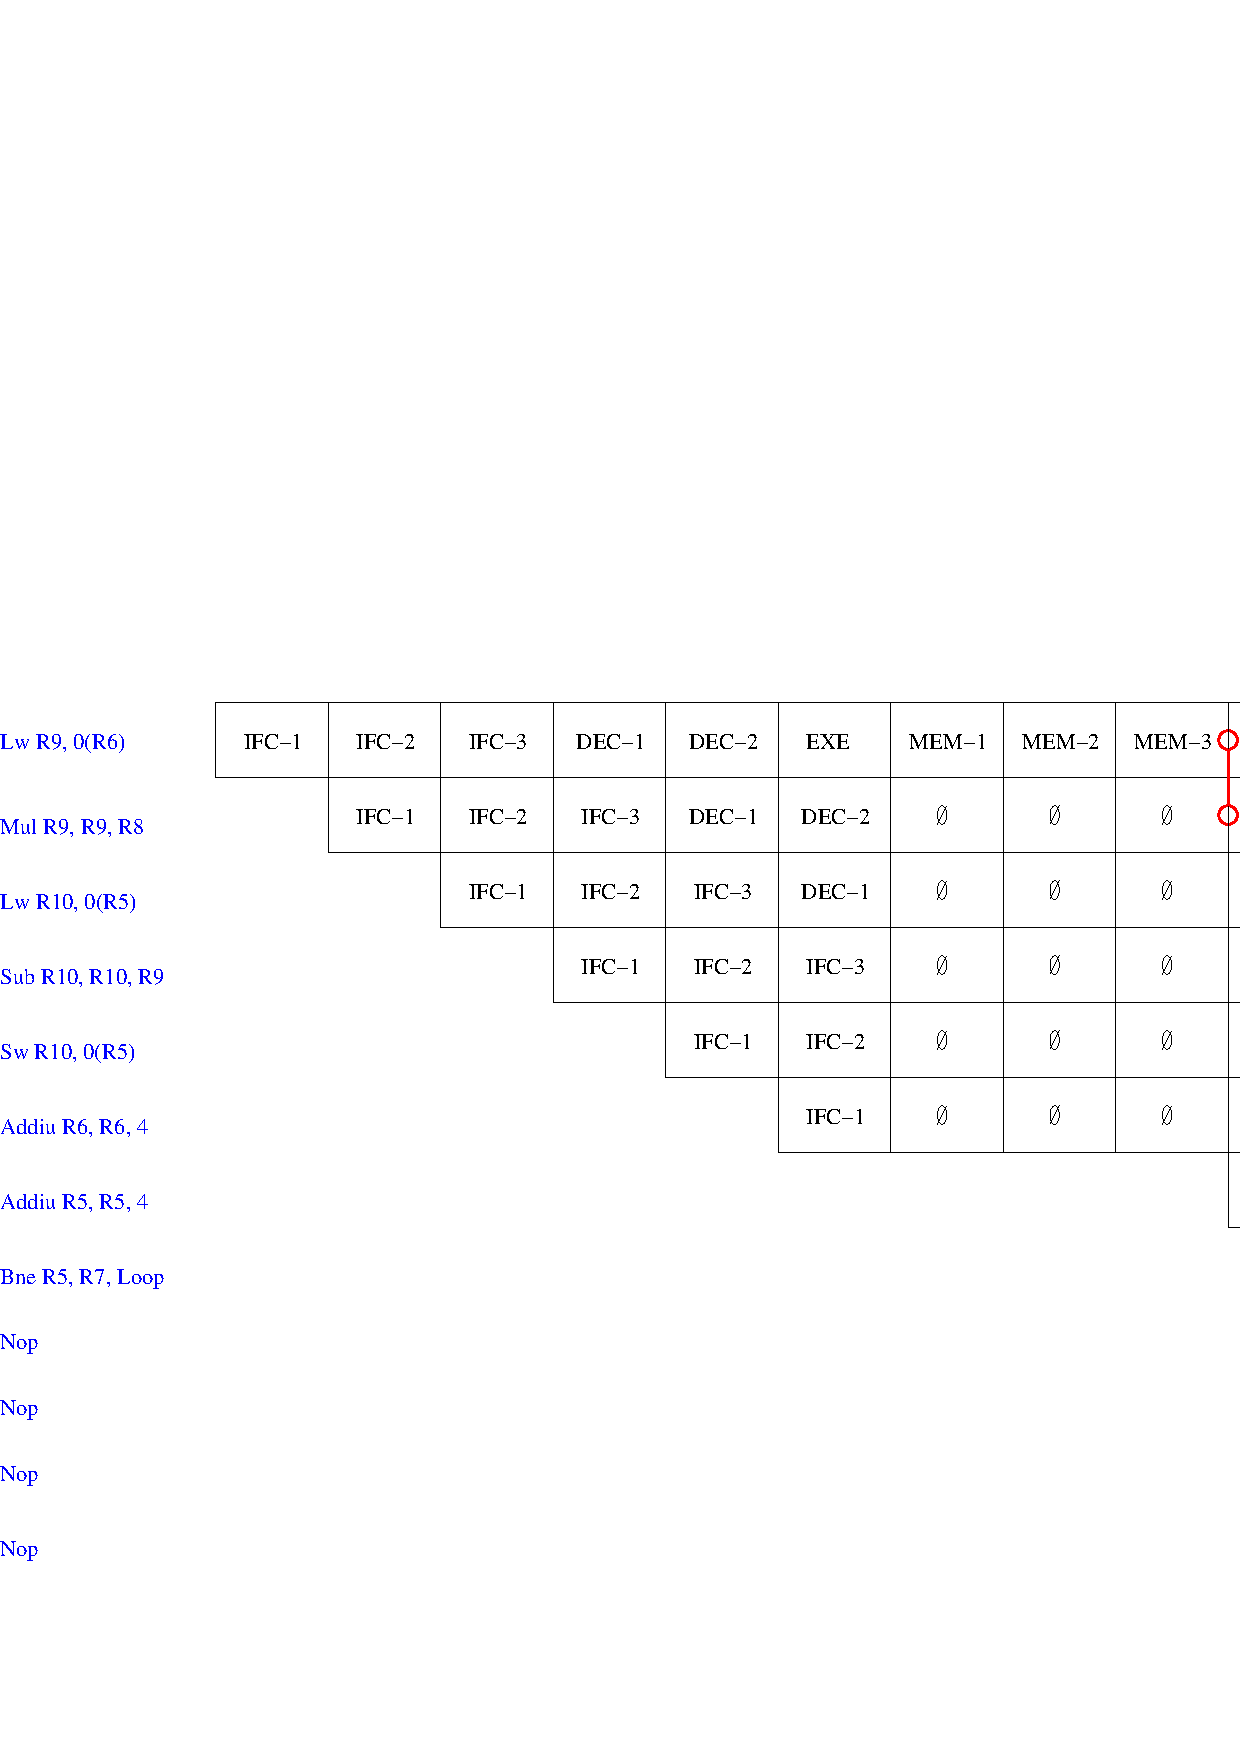
\includegraphics[scale=0.7]{figures/correction-analyse-simplifiee.jpg}
  \end{center}

\end{correction}

%
% reordonnancement
%

\section{R\'eordonnancement}

R\'eordonner le code assembleur de la boucle de mani\`ere \`a \'eviter
au maximum les cycles de gel et les cycles perdus dans les \textit{delay slots}.

Combien de cycles sont d\'esormais n\'ecessaires \`a l'ex\'ecution d'une
it\'eration?

\begin{correction}

  \begin{verbatim}
  Loop:    Lb R10, 0(R6)

           Addiu R5, R5, 1
           Addiu R6, R6, 1

           Beq R10, R0, EndLoop
           Nop

           Bne R6, R16, Loop
           Sb R10, -1(R5)
  \end{verbatim}

  Il faut d\'esormais \textbf{7} cycles pour l'ex\'ecution d'une it\'eration.
  Il ne reste plus de cycles de gel, n\'eanmoins il subsiste un
  \textit{delay slot} non utilis\'e.

\end{correction}

%
% analyse detaillee
%

\section{Analyse Detaill\'ee}

Donner un sch\'ema detaill\'e de l'ex\'ecution de la s\'equence d'instructions
suivante dans le pipeline classique MIPS 5 \'etages:

\begin{verbatim}
Lw R3, 0(R5)
Add R5, R1, R3
\end{verbatim}

\begin{correction}

  \begin{center}
    \includegraphics[scale=0.7]{figures/correction-analyse-detaillee.jpg}
  \end{center}

\end{correction}

%
% pipeline
%

\section{Pipeline}

On consid\`ere le processeur pipeline P construit autour d'un pipeline
\`a 7 \'etages.

En effet, l'\'etage IFC a \'et\'e d\'ecoup\'e: l'acc\`es m\'emoire commence
en IFC-1 et se termine en IFC-2.

De plus l'\'etage DEC a \'egalement \'et\'e d\'ecoup\'e. L'\'etage
DEC-1 d\'ecode et extrait les op\'erandes alors que l\'etage DEC-2 calcule
l'adresse de l'instruction suivante incluant bien entendu la comparaison
des op\'erandes dans le cas d'un branchement conditionnel.

\begin{center}
  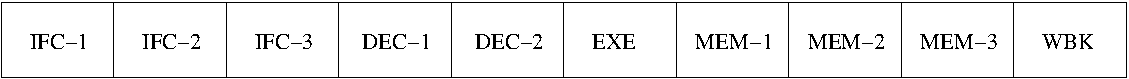
\includegraphics[scale=0.7]{figures/pipeline.jpg}
\end{center}

Combien de bypasses existent-ils sur ce processeur?

Representer ces bypasses sur un schema simplfi\'e?

Donner un exemple de code mettant en \'evidence chacun de ces bypasses.

\begin{correction}

  Il y a exactement \textbf{5} bypasses.

  \begin{center}
    \includegraphics[scale=0.7]{figures/correction-pipeline.jpg}
  \end{center}

  \begin{enumerate}
    \item
      \begin{verbatim}
	Add R3, R2, R1
	Add R5, R4, R3
      \end{verbatim}
    \item
      \begin{verbatim}
	Add R3, R2, R1
	Nop
	Beq R3, R0, Loop
      \end{verbatim}
    \item
      \begin{verbatim}
	Lw R3, 0(R5)
	Nop
	Add R5, R4, R3
      \end{verbatim}
    \item
      \begin{verbatim}
	Lw R3, 0(R5)
	Nop
	Nop
	Beq R3, R0, Loop
      \end{verbatim}
    \item
      \begin{verbatim}
	Lw R3, 0(R5)
	Nop
	Nop
	Nop
	Beq R3, R0, Loop
      \end{verbatim}
  \end{enumerate}

  \`A noter que la s\'equence:

  \begin{verbatim}
    Add R3, R2, R1
    Nop
    Nop
    Beq R3, R0, Loop  
  \end{verbatim}

  utilise le bypass num\'ero \textbf{4}.

\end{correction}

%
% optimisations
%

\section{Optimisations}

Modifier le code assembleur originel de la fonction \textbf{strncpy} de
mani\`ere \`a ce qu'il soit ex\'ecutable sur le processeur P.

Puis effectuer les optimisations suivantes sur la boucle du code
pr\'ec\'edemment obtenu:

\begin{itemize}
  \item
    R\'eordonnancement.
  \item
    Loop Unrolling.
\end{itemize}

Pour chacune de ces optimisations, vous devrez calculer le nombre de cycles
n\'ecessaire au traitement d'un \'el\'ement de la cha\^ine.

\begin{correction}

  Voici le code modifi\'e de mani\`ere \`a \^etre ex\'ecutable sur le
  processeur P.

  Il faut tout simplement prendre en compte les \textit{delay slots}.

  \begin{verbatim}
           Lw R5, 0(R29)
           Lw R6, 4(R29)
           Lw R7, 8(R29)

           Add R2, R5, R0

           Add R16, R6, R7

  Loop:    Lb R10, 0(R6)
           Beq R10, R0, EndLoop
           Nop
           Nop

           Sb R10, 0(R5)

           Addiu R5, R5, 1
           Addiu R6, R6, 1

           Bne R6, R16, Loop
           Nop
           Nop

  EndLoop: Sb R0, 0(R5)

           Jr R31
           Nop
           Nop
  \end{verbatim}

  \textbf{R\'eordonnancement}

  \begin{verbatim}
  Loop:    Lb R10, 0(R6)

           Addiu R5, R5, 1
           Addiu R6, R6, 1

           Beq R10, R0, EndLoop
           Nop
           Nop

           Bne R6, R16, Loop
           Sb R10, -1(R5)
           Nop
  \end{verbatim}

  \textbf{9} cycles sont n\'ecessaires \`a l'ex\'ecution de cette boucle et
  donc au traitement d'un \'el\'ement.

  \textbf{Loop Unrolling}

  \begin{verbatim}
  Loop:    Lb R10, 0(R6)
           Lb R11, 1(R6)

           Addiu R5, R5, 2

           Beq R10, R0, EndLoop
           Addiu R6, R6, 2
           Nop

           Bne R6, R16, Loop
           Sb R10, -2(R5)
	   Sb R11, -1(R5)
  \end{verbatim}

  \textbf{9} cycles sont n\'ecessaires \`a l'ex\'ecution de cette boucle.
  N\'eanmoins, le nombre de \textit{delay slots} a nettement diminu\'e de
  3 \`a 1.

  \'Etant donn\'e que deux caract\`eres de la cha\^ne sont trait\'es tous
  les \textbf{9} cycles, un caract\`ere est en moyenne trait\'e tous les
  \textbf{4.5} cycles.

\end{correction}

\end{document}
